%==============================================================================
\section{CCM Tools Component Model}
\label{section:CcmtoolsComponentModel}
%==============================================================================

A component type is a specific, named collection of features that can be
described by an {\bf Interface Definition Language} (IDL) and encapsulates its
internal representation and implementation.

\begin{figure}[htbp]
	\begin{center}
		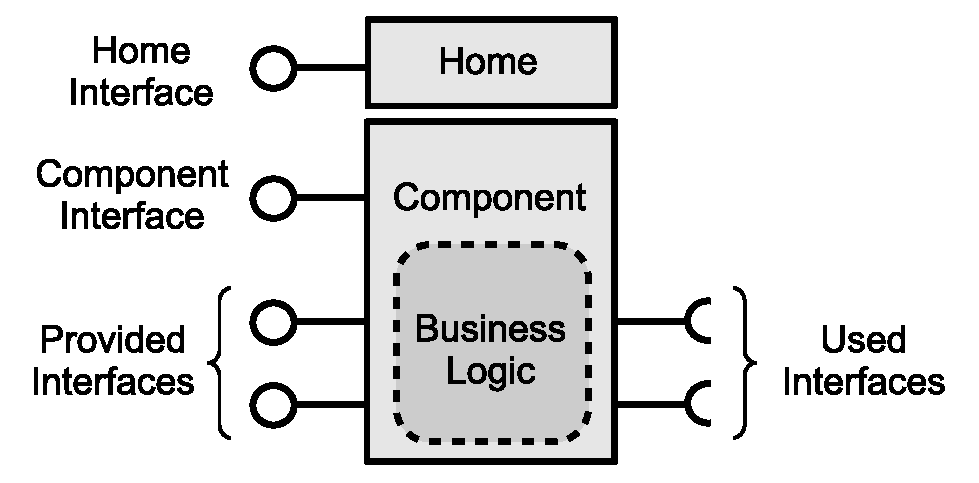
\includegraphics[height=5cm,angle=0] {figures/CcmtoolsComponent}
		\caption{ CCM Tools component model.}
		\label{figure:CcmtoolsComponentModel}
  	\end{center}
\end{figure}


To describe software components, some additional keywords have been 
introduced to the Interface Definition Language (IDL). 
A component definition may contain the following surface features:
\begin{itemize}
\item Attributes  
\item Supported interfaces
\item Provides interfaces 
\item Used interfaces
\end{itemize}

Additionally, a home definition must be declared for every component
type. These component homes act as a factory for component instances.

\vspace{2mm}
Example:
\begin{verbatim}
    #include <world/CommonInterface.idl>
    #include <world/FirstInterface.idl>
    #include <world/SecondInterface.idl>

    module world
    {
        /*
         * A component description collects zero or more surface 
         * features to a new component type.
         */
        component SimpleComponent supports CommonInterface
        {
            /*
             * Supported interfaces can be used to add attributes and
             * operations to the equivalent component interface (it's 
             * a kind of interface inheritance).
             */
             
        	    /* 
        	     * Component attributes can be used to configure a
        	     * particular component instance, and are added to the
        	     * equivalent component interface.
        	     */
            attribute string version;
            
            /*
             * Provided interfaces must be implemented by the component's
             * business logic, and can be used by clients or other 
             * components.
             */
            provides FirstInterface first;

            /*
             * Used interfaces are implemented by another component. 
             * A component's business logic call operations on used
             * interfaces to communicate with other component instances.
             */
            uses SecondInterface second;
        };        
        
        /*
         * A home definition must be declared for every component type.
         */
        home SimpleComponentHome manages SimpleComponent
        {        
            /*
             * A home definition may contain zero or more factory
             * definitions. Each factory method can be used to
             * create an instance of the given componet type.
             */
            factory createWithVersion(in string version);
        };
    }; // end of module world
\end{verbatim}

A component description will be transformed into a set of equivalent 
interfaces which define the component's API for clients and other component instances.
In the following sections these equivalent interfaces will be described 
in detail.


%------------------------------------------------------------------------------
\subsection{Home Interface}
%------------------------------------------------------------------------------



%------------------------------------------------------------------------------
\subsection{Component Interface}
%------------------------------------------------------------------------------


The component home interface implicitly provides a {\tt create()} operation
to create instances of the managed component type.







%------------------------------------------------------------------------------
\subsection{Provided Interfaces}
%------------------------------------------------------------------------------


%------------------------------------------------------------------------------
\subsection{Used Interfaces}
%------------------------------------------------------------------------------




\newpage
